\chapter{绪论}

\section{引言}
子痫前期(preeclampsia, PE)又作先兆子痫,是孕妇妊娠期特有的一种多系统进展性疾病, 与妊娠期高血压(gestational hypertension)、子痫(eclampsia)、
慢性高血压并发子痫前期(chronic hypertension with superimposed preeclampsia)以及妊娠合并慢性高血压(chronic hypertension)统称妊娠期
高血压疾病(hypertension disorders of pregnancy, HDP)\cite{OAG9,HDASOM,2000s1},
子痫前期临床表现的显著特点是原发性高血压与蛋白尿。
近年来,世界卫生组织对子痫前期的涵盖范围进行了进一步的拓展,将其定义为:在妊娠20周后出现新发(原发)高血压,在两次间隔$4h$或$4h$以上的血压测定中,收缩压≥$140mmHg$和(或)
舒张压≥$90mmHg$,且伴有下列任一项或多项\cite{OAG9,FIGO}:
1.孕妇出现蛋白尿症状,其尿蛋白≥$300mg/24h$,或尿蛋白/肌酸酐比值≥$30mg/mol$,或随机尿蛋白≥(+);
2.孕妇无尿蛋白但伴有以下任一器官或系统功能紊乱、受累受损:心、肺(肺水肿)、肝(血清转氨酶水平为正常值2倍以上)、肾(血肌酐水平大于$1.1mg/dl$
或为正常值2倍以上)等重要器官,或血液系统(血小板<$100 \times 10^{9}/L$等)、消化系统、神经系统的异常改变等;
3.胎盘-胎儿受到累及,出现生长受限、脐动脉多普勒分析检测异常、死胎等。

妊娠期高血压疾病可引起严重的母胎并发症,是孕产妇和围产儿病死率升高的主要原因\cite{OAG9}。
据世界卫生组织统计,子痫前期在孕妇中发病率高达5\%-10\%,是除体内大出血外孕妇死亡的第二大危险因素\cite{LCT2006},每年可导致全球范围内约76 000名孕妇死亡,并进一步导致约500 000
名胎儿/婴儿的死亡\cite{DAM2015,LCT2006},如\autoref{fig:dhd}所示。为推广普及人们对危及母婴生命安全的子痫前期的认知,同时教育女性了解她们当前及长期的健康风险,
全球孕妇保健组织自2017年起将每年的5月22日确定为世界子痫日(world preeclampsia day)。
\begin{figure}[htbp]
    \centering
    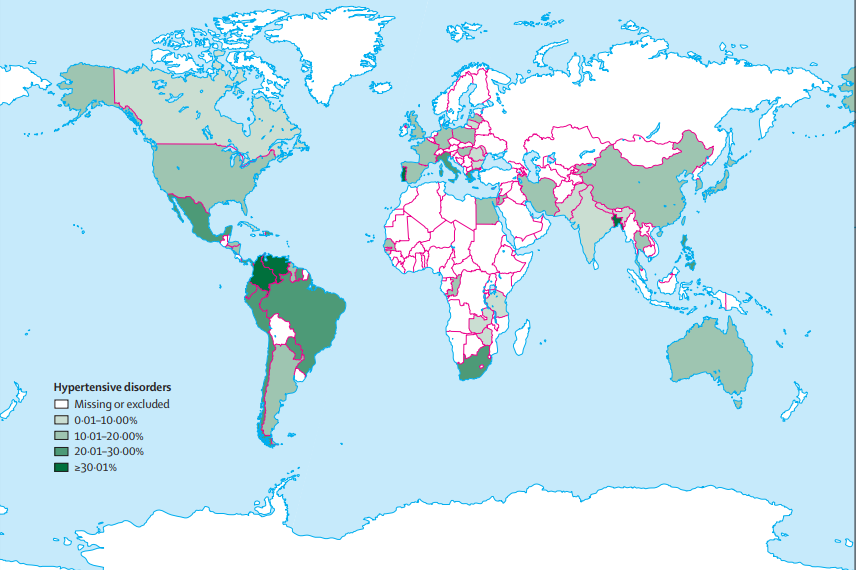
\includegraphics[width=.65\linewidth]{intro/dhd}
    \caption[因妊娠期高血压疾病死亡孕妇的国家分布比例]{\label{fig:dhd}因妊娠期高血压疾病死亡孕妇的国家分布比例\cite{LCT2006}}
\end{figure}

就现阶段我国国情而言,由于人口基数大、人口出生率较高,导致每年妊娠孕妇数及新生儿数总量巨大\cite{nbs2022}。
最新地区人口普查信息显示\cite{zjtjj2022},妇女峰值生育率微幅下降、高峰年龄区间后移并缩短,同时,妇女晚育现象比较普遍,自全面开放二孩政策后,二孩、多孩生育率持续回升。而临床研究已经证实,
高龄与多次妊娠均属于可能导致子痫前期的风险因素,会增加孕妇子痫前期的患病可能\cite{Duckitt2005,FIGO,Yogev2010,Poon2010,Lee2000,Coonrod1995,Robillard1993}。
因此,实现子痫前期的预测与快速有效的医学诊断乃至精确治疗与干预,可以有效保障孕妇及围产儿的生命健康安全,具有重大的临床应用价值。
\section{子痫前期概述}
\subsection{病因及发病机制}
截止目前,医学界对子痫前期的病因与发病机制尚未完全明确,相关研究还在继续进行之中。但得到公认的一点是,子痫前期病发具有异质性,多因素、多机制及多通路均对子痫前期的发病有所影响,不能仅以“一元论”的观点对待。
目前临床对子痫前期的病因和发病机制的研究可以概括如下:

一、主流学说

目前临床最为普遍接受的子痫前期是由子宫螺旋小动脉重铸不足导致的,
该学说认为子痫前期的发病与妊娠早期胎盘功能紊乱密切相关\cite{OAG9,Duvekot2010,2009ix},其作用机制可以概括为两个阶段,如\autoref{fig:ppp}所示。
在第一阶段,孕妇子宫螺旋动脉重构受损、出现重铸障碍,绒毛外滋养细胞浸润能力受损,导致胎盘缺血、缺氧,释放多种胎盘因子,该阶段无明显临床现象;在第二阶段,各种胎盘因子进入母体血液循环,血管阻力增大,胎盘灌注减少,
促进系统性炎症反应的激活及血管内皮损伤引起子痫前期-子痫多样化的临床表现。
\begin{figure}[htbp]
    \centering
    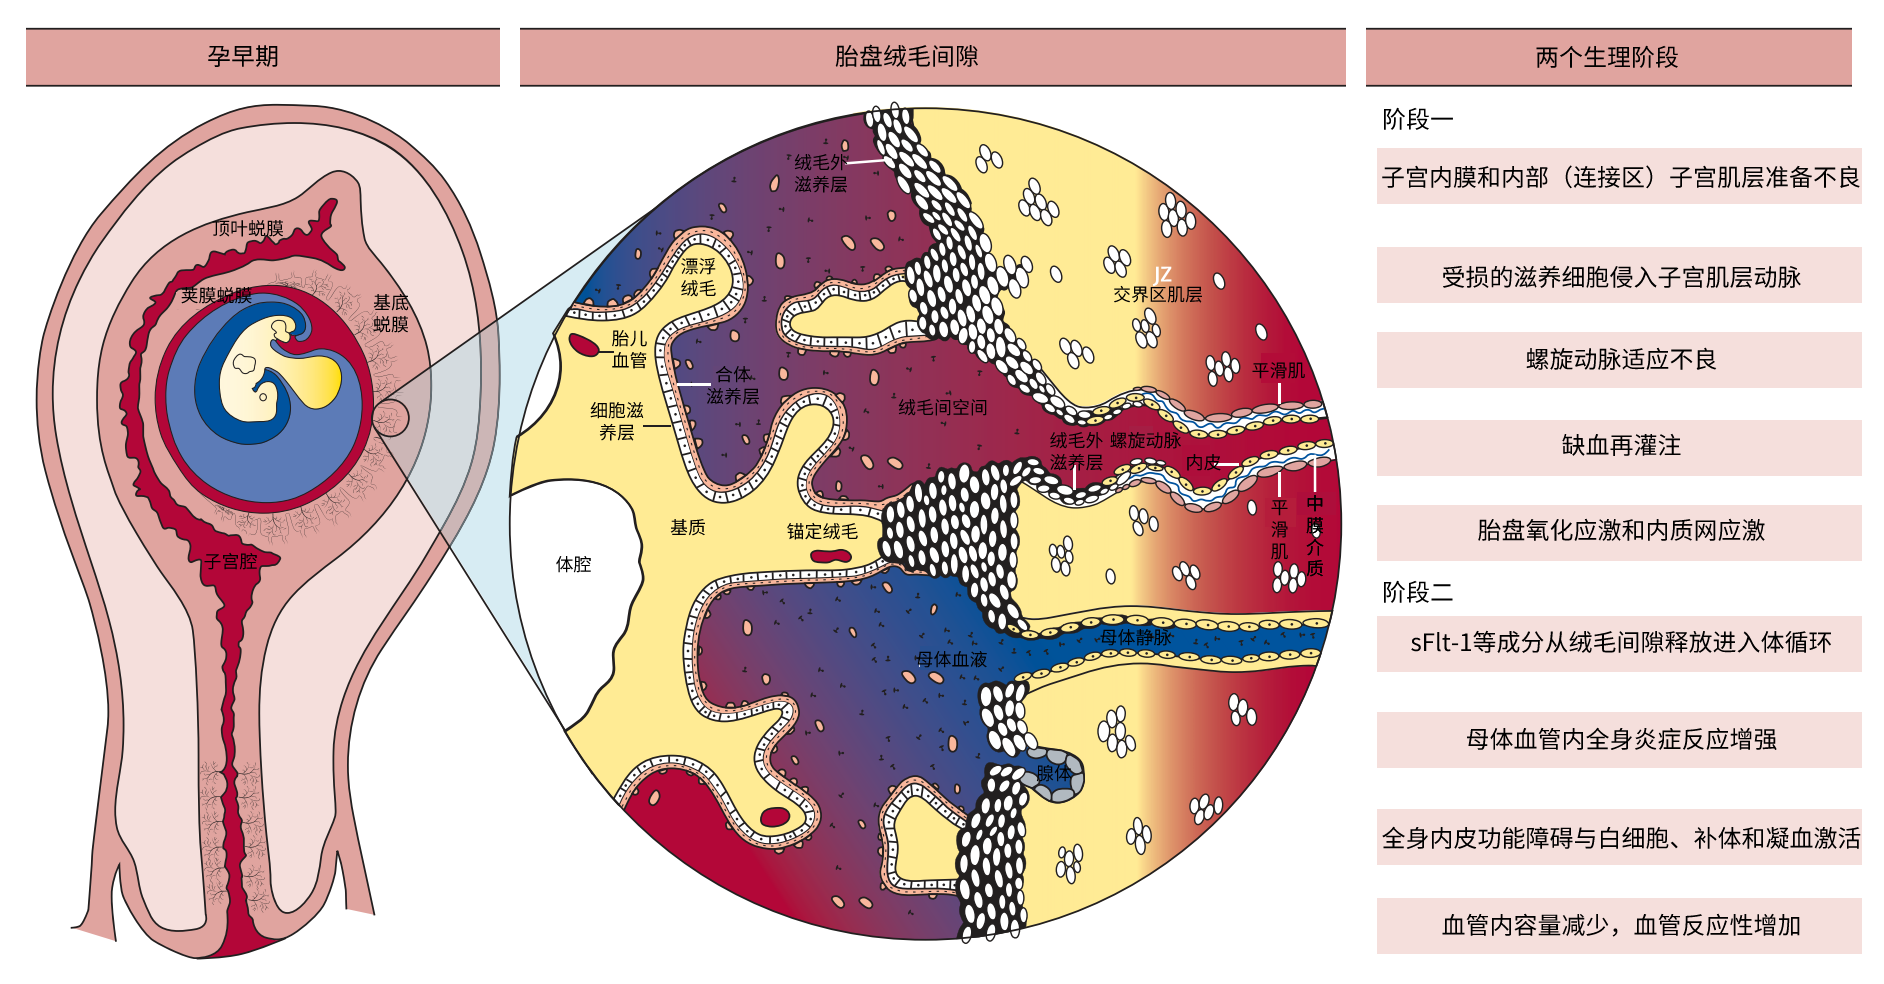
\includegraphics[width=\linewidth]{intro/ppp}
    \caption[子宫螺旋小动脉重铸不足学说认为的子痫前期发病机制]{\label{fig:ppp}子宫螺旋小动脉重铸不足学说认为的子痫前期发病机制\cite{Duvekot2010,2009ix}。}
\end{figure}

二、其他学说

除上述学说外,学者们还提出了其他多种子痫前期可能的发病机制,包括炎症免疫过度激活学说、血管内皮细胞损伤及前列腺素合成失调学说及遗传学说等。
炎症免疫过度激活学说认为子痫前期是母系-父系免疫适应不良导致的,即胎儿胎盘具有的半抗原性移植体特性导致同种异体移植排斥,最终引起的母系同种免疫反应从而诱发子痫前期\cite{Sibai2005,OAG9,Shi2006,Moffett2002}。
血管内皮细胞损伤及前列腺素合成失调观点认为,当血管内皮细胞出现损伤后,将进一步导致前列腺素合成失调\cite{OAG9,Sibai2005}。它使扩血管物质如一氧化氮(NO)、前列环素(PGI2),合成减少,而缩血管物质如内皮素(ET)、
血栓素(TXA2)等合成增加,从而促进血管痉挛引发子痫前期。遗传学说则是以子痫前期具有家族倾向性的临床现象为基础\cite{OAG9,Sibai2005,Ge2013}。
近年来,学者们还相继提出一些新的可能引起子痫前期的学术观点,如胎盘因子学说\cite{Shi2006}等。同时一些临床研究也发现,多种营养因素如低白蛋白血症、钙、镁、锌、硒等缺乏与子痫前期发生发展
可能有关\cite{OAG9}。但此类学说与假设仍需进一步临床研究与理论研究来证实。

\section{子痫前期监测的研究现状}
现代医学对子痫前期的认知经历了漫长的探索\cite{BJOG2016}。早在古希腊希波克拉底(Hippocrates)时代(约公元前460-370年),医学界就对子痫的症状有一定的认识。但直至18世纪,医学界才将子痫与癫痫加以区分对待。
19世纪中叶,医学界开始认识到子痫之前存在一个前驱状态。此外,法国医生Pierre Rayer首次描述了子痫孕妇的蛋白尿症状,英国医生John Lever更进一步证实了蛋白尿与子痫发病的特异性关系。
20世纪初,尿液分析与血压测量开始用于子痫的诊断,同时,进一步细化的子痫前期的相关概念开始出现。20世纪中后叶,由于医学诊断技术的发展,多种新的检测指标与技术不断被引入子痫及子痫前期的识别诊断中。
进入21世纪后,由于智能化设备的发展,基于医学大数据的人工智能相关研究又成为了新的热点。

本小节将从现阶段临床对子痫前期发生评估的常用参数、医用检测设备及新兴人工智能检测技术等三方面对子痫前期的临床监测进行介绍。
\subsection{检测参数}
现阶段,临床使用的子痫前期的检测参数可概括为风险因子(risk factors)与生物标志物(biomarkers)等两大类。

一、风险因子筛查

已有研究表明,许多孕妇自身风险因子与子痫前期的发生密切相关\cite{Magee2008,FIGO,Lowe2015,Heazell2010}。临床医生往往会以量表问卷的形式向孕妇采集这些信息,
对孕妇罹患子痫前期的可能进行初筛\cite{risks},如\autoref{fig:risk}所示。常见的子痫前期风险因子及其可能影响如\autoref{tab:riskfactors}所示。
\begin{figure}[htbp]
    \centering
    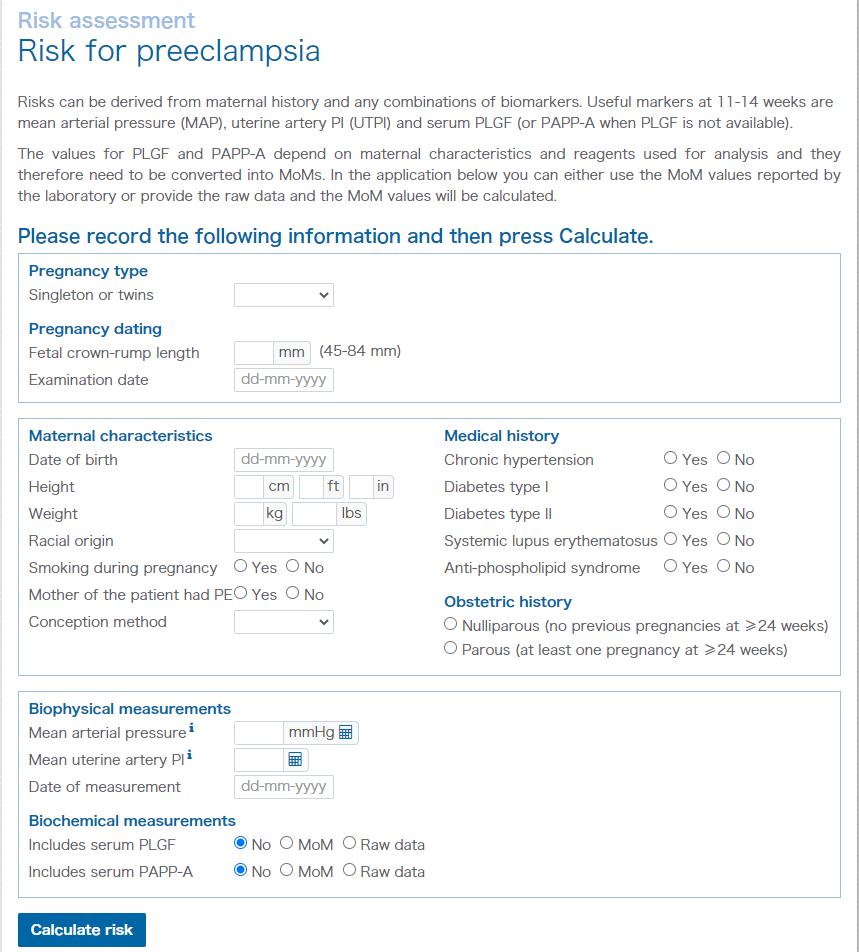
\includegraphics[width=.5\linewidth]{intro/risk}
    \caption[英国胎儿医学基金会网站给出的子痫前期风险因子评估量表]{\label{fig:risk}英国胎儿医学基金会网站给出的子痫前期风险因子评估量表\cite{risks}}
\end{figure}

\begin{center}
    \zihao{5}
	\begin{longtable}{m{2.5cm}<{\centering}m{12cm}<{\centering}}
		\caption{\label{tab:riskfactors}常见的子痫前期风险因子}\\
        \toprule
        \textbf{风险因子} & \textbf{可能影响}\\
        \midrule
        \endfirsthead
        \caption[]{(续)}\\
        \midrule
        \textbf{风险因子} & \textbf{可能影响}\\
        \midrule
        \endhead 
        \midrule
        \endfoot
        \bottomrule
        \endlastfoot
        产妇年龄&  子痫前期的发病可能随年龄升高而增加\cite{Duckitt2005,FIGO,Yogev2010,Poon2010}。    \\
        胎产次/既往史&    首次分娩产妇罹患子痫前期的概率比未患有子痫前期既往史的二胎孕妇风险更大\cite{Lee2000,Duckitt2005,Coonrod1995,Robillard1993,Sonia2009},。   \\
        妊娠间隔 & 多次妊娠间隔时间过长或过短都会在一定程度上增加PE发生的风险\cite{Rousso2002,Duckitt2005,Conde2007,Mignini2016,Rolv2002}。\\
        辅助生殖 & 孕妇通过辅助生殖技术受孕时,子痫前期患病可能增加\cite{Jackson2004,Trogstad2009,Martin2016}。\\
        家族史 & 子痫前期在一定程度上显现出家族性易感性\cite{ARNGRIMSSON1990,OAG9,Williams2011,Cincotta1998,FIGO}\\
        肥胖 & 若孕妇出现肥胖症状($BMI>30kg/m^2$),其患病风险会增加\cite{Duckitt2005,Williams2011,FIGO,Zintzaras2006,Sebire2001}。\\
        种族&不同民族、区域、肤色的孕妇其子痫患病可能会有一定的差异\cite{Ghosh2014,Khalil2013}。\\
        并发症 & 当孕妇自身已患有某些疾病或感染某些症状时,其患病可能也会增加\cite{FIGO,Ray2016,OAG9,Lee2000,Garner1990,Martinell1990,Stamilio2000,Dreyfus2001,Marchetti2016}。\\
	\end{longtable}
\end{center}
\raggedbottom
二、生物标志物筛查

筛查子痫前期的另一种方法是基于贝叶斯定理,将孕妇的PE风险因子、特定病史的先验风险及其多项生物物理、生物化学检测结果相结合,从而估计其PE患病风险\cite{FIGO}。
这一过程即为参数估计中的极大后验概率估计
(maximum aposterori,MAP),即按照观测值判断当前值x最可能属于哪一类进行分类决策\cite{Qiu2012}。基于MAP的二分类过程可以表示为
\begin{equation}
    \label{equ:maxap}
    H_{x}=
    \left \{
    \begin{aligned}
        &H_{1}, \text P(H_{1}|x)&>P(H_{0}|x), \\
        &H_{0}, \text P(H_{1}|x)&<P(H_{0}|x),
    \end{aligned}
    \right.  
\end{equation}
其中,$P(H|x)$为观测值x属于$H$的后验概率,选出从观测值x所有类别中选出后验概率最大的,即为观测值所属类别。

上述筛选过程中孕妇的生理、生化检测结果统称为生物标志物。其中,生理参数主要包括血压、子宫动脉搏动指数等;生化参数则种类繁多、新参数层出不穷\cite{Rene2008,Zhong2015,Zeisler2016,Rana2012}。
这里选取血清妊娠相关蛋白A(Pregnancy associated plasma protein A,PAPP-A)与血清胎盘成长因子(placental growth factor,PLGF)为代表进行介绍。

1. 血压

由于PE是妊娠期高血压疾病的一种,血压对PE的影响和意义不言而喻\cite{OAG9,HDASOM,2000s1}。血压值一直以来是临床用以对PE监测、诊断的重要指标。测量血压时,孕妇同一手臂应至少测量两次,收缩压>140mmhg和或舒张压>90mmhg定义为高血压。
对首次发现血压升高的孕妇,应至少间隔4小时后再次测量确认\cite{OAG9}。除基本的收缩压(systolic blood pressure,SBP)、
舒张压(diastolic blood pressure,DBP)外,国际妇产科联盟更是推荐使用平均动脉压(mean arterial pressure,MAP)作为实际标定诊断中的筛查指标,其计算方法如\autoref{equ:map}所示\cite{FIGO}
\begin{equation}
    \label{equ:map}
    MAP=DBP+(SBP-DBP)/3
\end{equation}
Leona C.Y. Poon等人对5590名单胎孕妇的一项研究表明,当单独使用MAP进行检测时,PE的检测率为38\%;当结合孕妇病史等因素时,PE检出率可达63\%,假阳性率为10\%\cite{Poon2008}。
Stamilio等人发现,孕妇第一次产前检查时出现MAP>90毫米汞柱与其PE患病的可能相关性显著\cite{Stamilio2000}。

2. 子宫动脉搏动指数

UTPI是国际妇产科联盟与妇产科超声学会所推荐的对PE进行筛查的参数之一\cite{FIGO,Sotiriadis2019}。\autoref{fig:utpi}展示了一例孕早期经腹多普勒超声检查子宫动脉的结果\cite{Sotiriadis2019}。
UTPI本质上也是一种血液动力学参数,其基本定义与MAP类似,是子宫动脉收缩期峰值流量$A$减去舒张末期流量$B$除以平均流量$M$\cite{Cnossen2008}:
\begin{equation}
    \label{equ:utpi}
    UTPI=\frac{A-B}{M}
\end{equation}
同时,常与UTPI一起检测的还有子宫动阻力动指数(Resistance index,RI)、子宫动脉(peak systolic to late diastolic ratio,S/D R)及切迹等参数\cite{Cnossen2008}。
\begin{figure}[htbp]
    \centering
    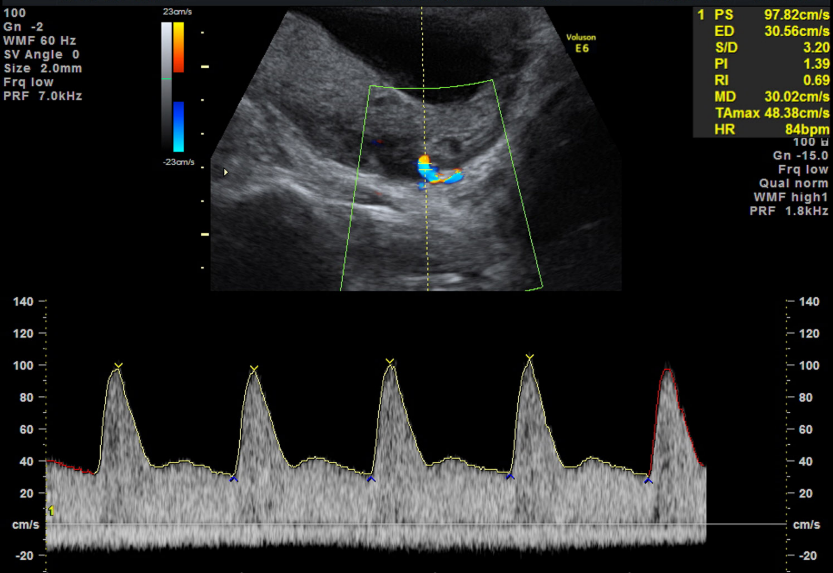
\includegraphics[width=.6\linewidth]{intro/utpi}
    \caption{\label{fig:utpi}孕早期经腹多普勒超声检查子宫动脉}
\end{figure}
Jeltsje S. Cnossen等人\cite{Cnossen2008}此前众多学者研究的回顾表明,在孕妇妊娠$11^{+0}-13^{+6}$周时,若子宫动脉多普勒血流检测发现UTPI上升或出现子宫动脉舒张早期切迹等现象,该孕妇PE患病的可能性将增加\cite{OAG9,Plasencia2008}。

3.血清妊娠相关蛋白A

PAPP-A是由细胞滋养层分泌的一种金属蛋白胰岛素生长因子结合蛋白,在胎盘的生长发育中起着重要的作用。PE已被证明与低水平的PAPP-A循环有关\cite{FIGO}。但相关临床研究表明,仅使用PAPP-A单指标无法准确预测PE\cite{Smith2002}。
因此,PAPP-A常与其他检测参数一起配合使用\cite{Poon2009,Tan2018,Ray2018}。 

4. 胎盘生长因子

PLGF是由绒毛状细胞滋养层膜细胞滋养层合成,是一种糖基化二聚糖蛋白,具有血管生成合血管修复的功能。临床研究显示,PLGF的血管生成功能在妊娠过程中会发挥很大作用,PLGF水平或其抑制受体水平的变化可能与PE的发生有关\cite{Levine2004,Ahmad2004}。
同时,临床证据表明,在孕早期患有PE的孕妇其PLGF的浓度较正常妊娠孕妇更低\cite{Chau2017}。

2019年,Duhig等人\cite{Duhig2019}对1019名疑似PE的孕妇进行了追踪实验,在整个实验期间一直持续性的进行PLGF水平检测。结果显示,针对实验组(n=573),PE诊断时间的中位数为4.1天,而对照组(n=446)这一数值仅为1.9天,证明PLGF可以有效的缩短PE确诊的时间。
2015年,Zhong等人\cite{Zhong2015}对多项血清生化指标在PE预测方面的性能进行了比较,结果显示,PLGF的综合性能优于其他诸如胎盘蛋白13(Plancenta protein 13,PP13)、PAPP-A
等其他血清生化指标。鉴于此,\textbf{FIGO组织特别将胎盘生长因子推荐为PE检测首选生化指标}\cite{FIGO}。

\subsection{检测设备}
一、标准医疗设备

目前临床所使用的PE筛查检测设备主要以检测生化标志物为主,国内外医疗器械公司均研发推出了一定的软硬件综合分析系统。但整体而言,国内医疗器械设备公司研发起步晚,较国外同类型设备而言,可检测指标数目较少。

1. 德国勃拉姆斯公司的产前检测设备

勃拉姆斯公司(B·R·A·H·M·S GmbH)一直致力于对各种生物标志物检测的研究中,其公司产品KRYPTOR GOLD与KRYPTOR compact PLUS\cite{B·R·A·H·M·S2021}可完成对AFP、Free $\beta$hCG、$\beta$hCG、PAPP-A、PlGF、
sFlt-1、uE3等在内的多种生物标志物的检测,
满足PE的早期筛查及诊断等多种应用场景,如\autoref{fig:B·R·A·H·M·S}所示。同时该公司还研发了一套Fast Screen pre I plus$^\text{TM}$综合软件分析系统,可结合检测结果对孕妇PE发病可能进行风险评估。

\begin{figure}[htbp]
    \centering
    \subfigure[KRYPTOR GOLD]{
    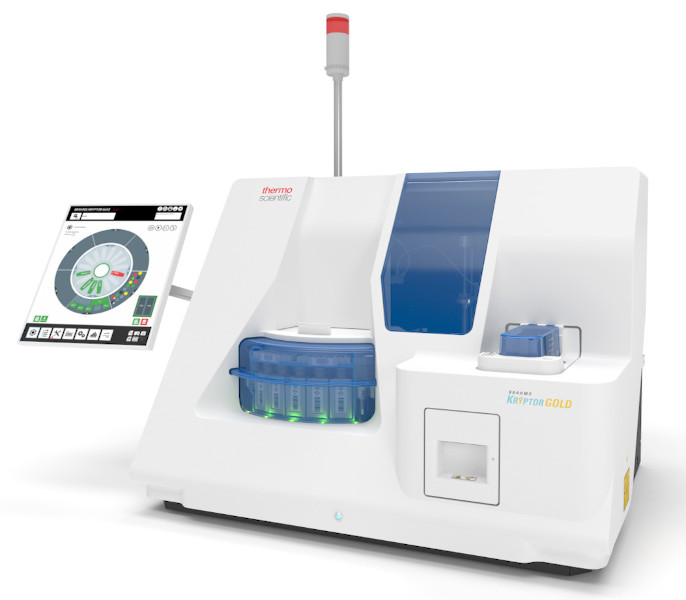
\includegraphics[width=5.5cm]{intro/brahms-kryptor-gold-686}
    }
    \quad
    \subfigure[KRYPTOR compact PLUS]{
    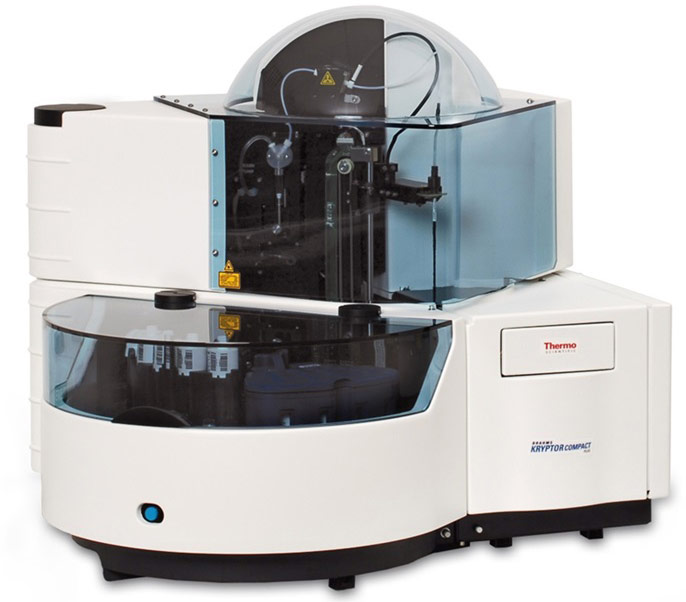
\includegraphics[width=5.5cm]{intro/brahms-kryptor-compact-plus-686}
    }
    \caption{\label{fig:B·R·A·H·M·S}勃拉姆斯公司KRYPTOR系列的两款检测设备}
\end{figure}
2.美国珀金埃尔默公司的产前检测设备

珀金埃尔默公司(PerkinElmer)提供全面的筛查和诊断解决方案组合,推进早期临床检测在成医疗领域的应用。该公司针对PE在内的多种孕期综合并发症提出了完整的检测方案,其AutoDELFIA系列、
VICTOR2系列及DELFIA Xpress系列的多款免疫荧光分析仪平台\cite{perkinelmer2021}均可完成对AFP、Free $\beta$hCG、$\beta$hCG、PAPP-A、PlGF、
sFlt-1、uE3等在内的PE生物标志物检测标定,如\autoref{fig:PerkinElmer}所示。此外,该公司位硬件检测设备配套研发了LifeCycle软件分析系统,实现了从样品接收-检验检测-风险评估-化验报告的全自动工作流程。
\begin{figure}[h]
    \centering
    \subfigure[VICTOR2 D荧光检测仪]{
    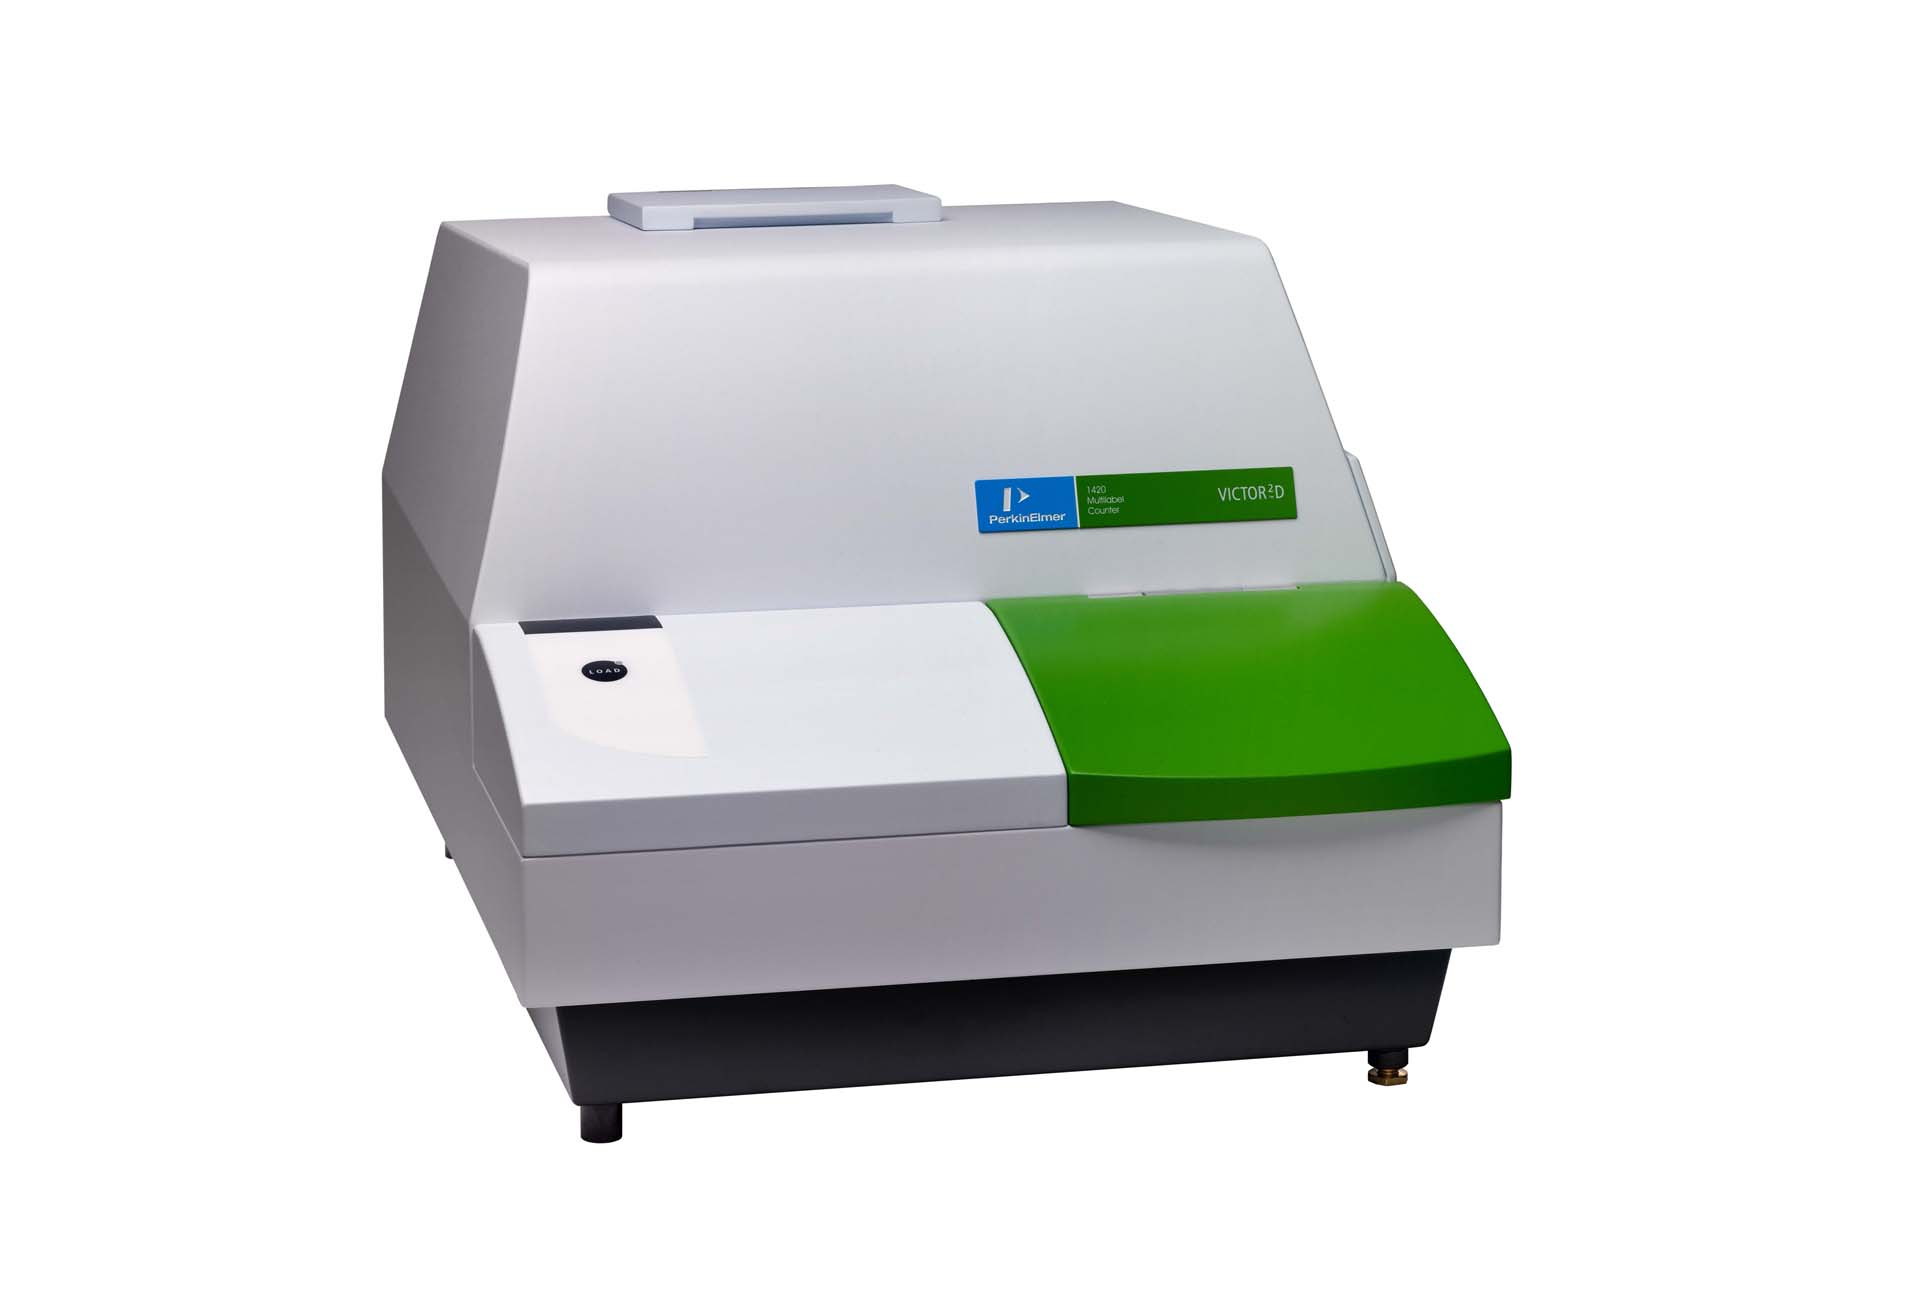
\includegraphics[width=5.5cm]{intro/Victor-2D-72ppi}
    }
    \quad
    \subfigure[DELFIA® Xpress免疫分析仪平台]{
    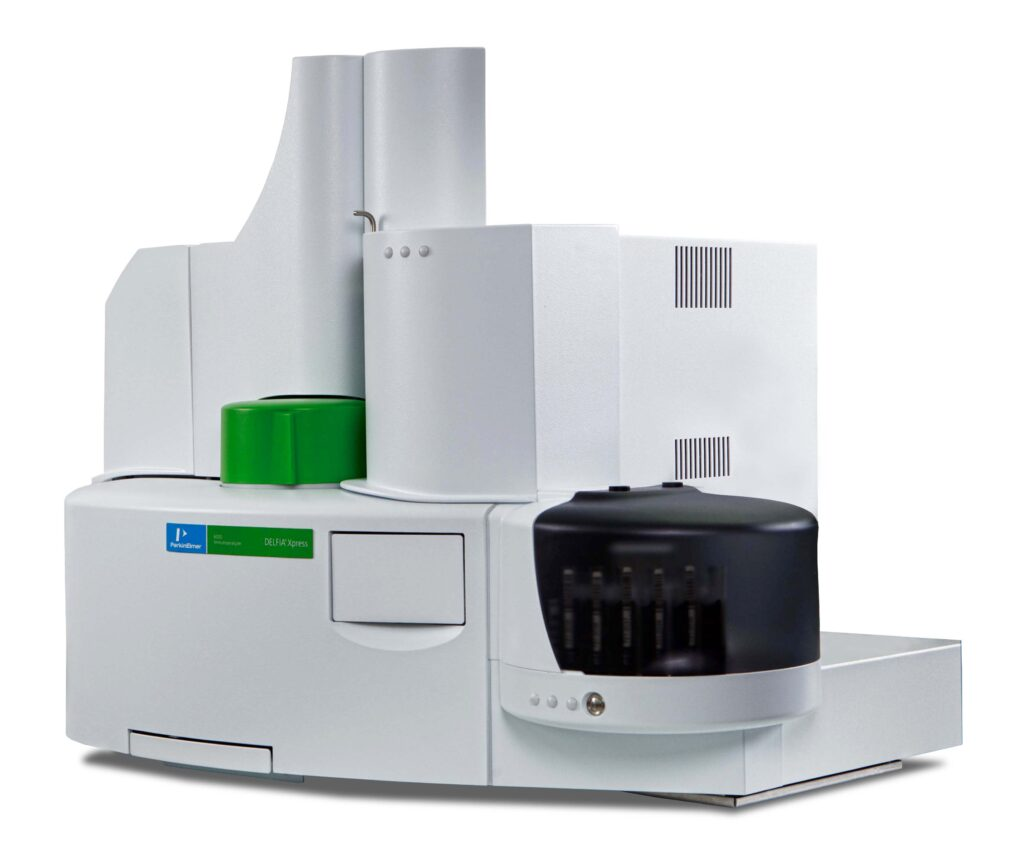
\includegraphics[width=5.5cm]{intro/dx}
    }
    \caption{\label{fig:PerkinElmer}珀金埃尔默公司的两款检测设备}
\end{figure}

3. 中国宁波奥丞生物科技有限公司的荧光检测设备

作为中国新兴的医疗器械设备公司,奥丞专注于从疾病早期发现、诊断、预防到监测,力求通过提供可靠、快速与便捷的体外诊断产品为诊疗提供精准的检测结果。
目前,奥丞公司的多款化学荧光免疫平台产品均支持对PE生物标记物PLGF、sFlt-1等两种指标的检测\cite{aucheer2021}。此外,奥丞还根据实际临床需求,
提供了微小型床边诊断设备与大型实验室标定两种类型的设备,如\autoref{fig:aucheer}所示。
\begin{figure}[h]
    \centering
    \subfigure[微流控荧光免疫定量检测系统 iSort300]{
    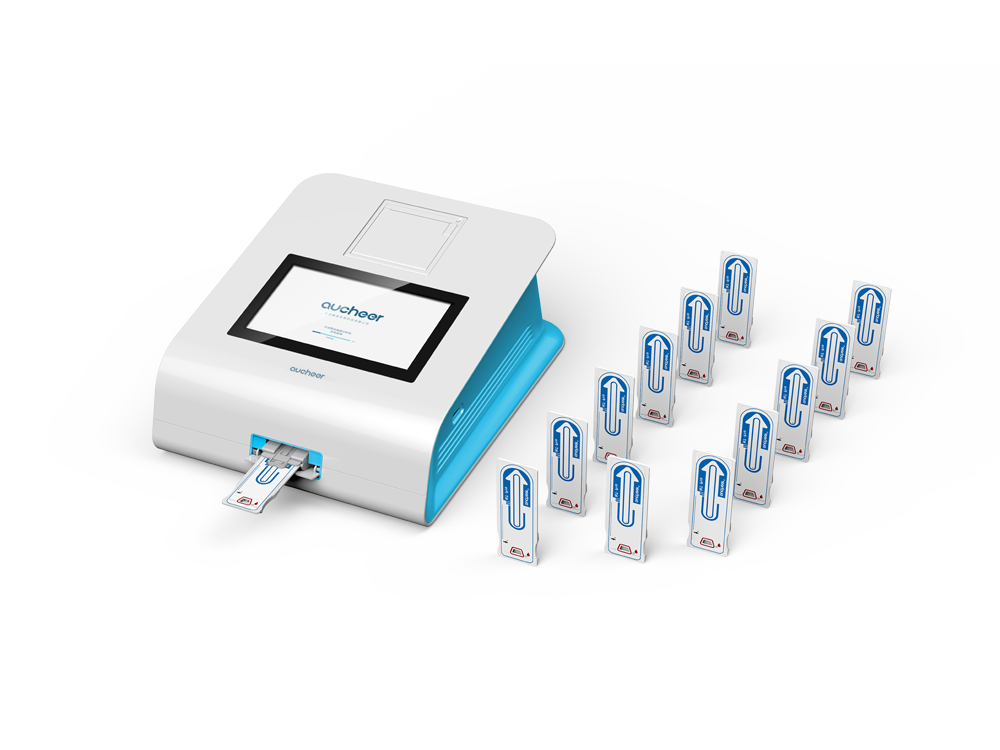
\includegraphics[width=5.5cm]{intro/isort300}
    }
    \quad
    \subfigure[全自动化学发光免疫检测系统 Shine i1910]{
    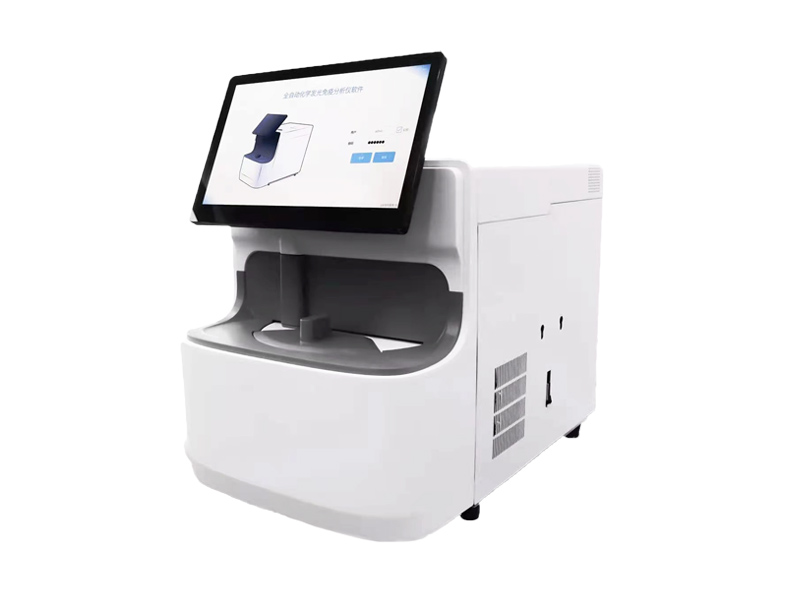
\includegraphics[width=5.5cm]{intro/shinei1910}
    }
    \caption{\label{fig:aucheer}奥丞生物科技公司的荧光免疫平台}
\end{figure}


二、微型智能设备

随着移动智能医疗和可穿戴式设备的发展,通过微型智能设备实现对PE相关指标的实时、动态、多场景检测也逐渐成为了新的研究热点。
2019年,Iuliana Marin等人\cite{Marin2019,Marin2020}通过一款智能腕部血压检测穿戴设备对孕妇的血压数据进行了监测,同时综合考虑孕妇的年龄、体重等风险因素,通过维特比动态规划算法(Viterbi algorithm),判断决策孕妇子痫前期
的患病可能,该系统原理框架图如\autoref{fig:mobile}所示。Iuliana Marin团队
通过对105名试验人员进行了测试,结果显示,最终的生成模型可以达到总体准确率80\%,敏感性为92.5\%,特异性为72\%\cite{Marin2019}。
\begin{figure}[htbp]
    \centering
    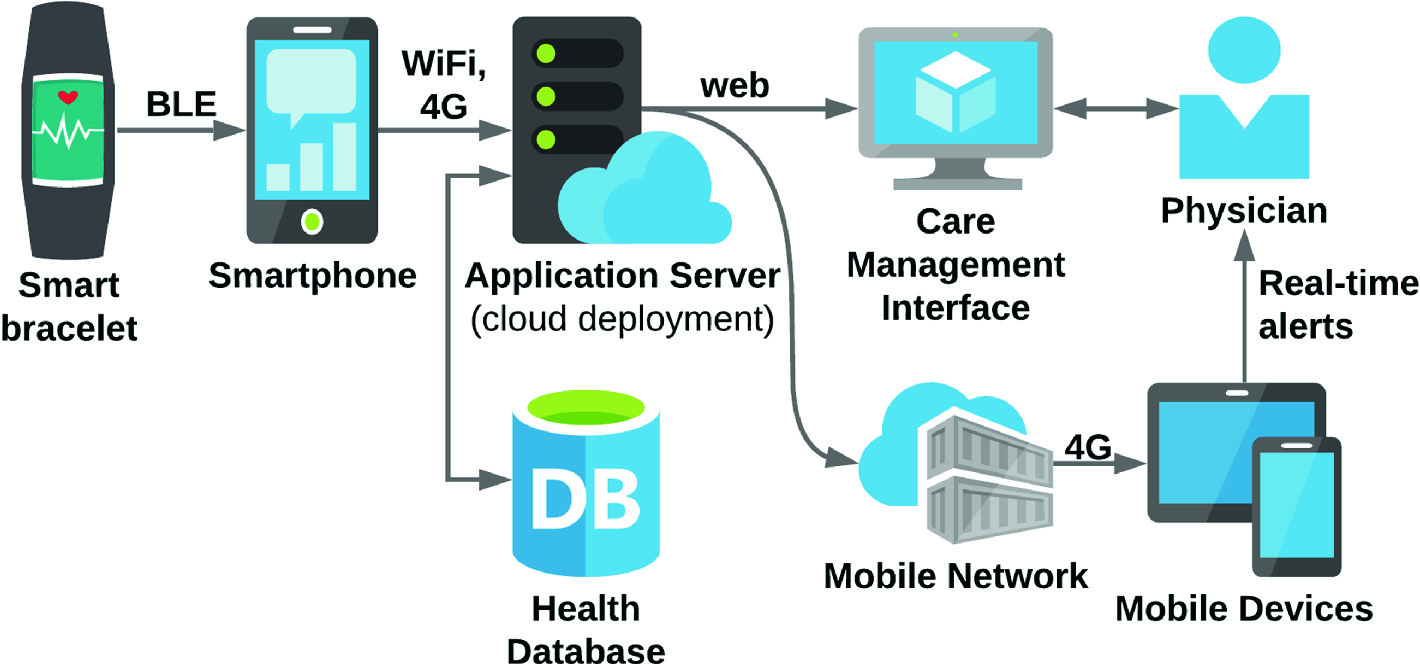
\includegraphics[width=.6\linewidth]{intro/mobile}
    \caption[基于智能穿戴设备的血压检测系统框架图]{\label{fig:mobile}基于智能穿戴设备的血压检测系统框架图\cite{Marin2019,Marin2020}}
\end{figure}
但整体而言,基于智能设备的PE检测设备仍处于研发阶段,能真正实现多场景检测的成熟的PE分析系统尚未出现。

\subsection{分析技术}
近年来,由于现代化设备的普遍使用致使医学检查过程各项数据激增,同时计算机领域人工智能技术的不断创新发展,相关研究者也开始尝试在子痫前期的识别、判断乃至预测等研究内容上引入人工智能技术。
利用人工智能技术分析前小节提到的各项风险因子、生理化学等参数一时间成为了炽手可热的多学科交叉研究点。

这些学者的研究可以分为数据挖掘与分析总结为两大类应用研究方向,即关联规则(Association Rule)挖掘方向与分类、聚类分析方向\cite{Mehta2016}。
关联规则挖掘力求发现多项数据之间的隐藏的逻辑与关系;分类分析是对通过现有数据建立模型预测新数据所属类别,聚类分析则是按照一定规则将所有数据分组,
使每组内的数据尽可能相似并有别于其他组数据\cite{Han2006}。
基于机器学习的PE研究可总结为\autoref{tab:AIinPE}。其中,数据集规模一栏按实验组人数+对照组人数或参与实验总人数的形式进行标注。

一、数据挖掘

在子痫前期的相关研究中,利用数据挖掘技术从血浆代谢物、蛋白质及$mRNA$等生化指标中筛选出与PE患病最为相关的成份一直是研究热点。这些研究往往都是在实现数据降维的同时揭示数据之间隐藏的联系。

2005年,Louise C. Kenny等人\cite{Kenny2005}从利用基因遗传算法(genetic programming,GP),从血浆中代谢物成份确定特异的成份来识别患有PE的孕妇。他们通过对受试孕妇(其中,患有PE的实验组$N_{PE}=87$,正常对照组$N_{Normal}=87$,下同)
的血浆成份分析后,通过GP训练出了仅使用三种代谢物峰值变量预测模型。预测模型可以有效区分患有PE与正常孕妇,其灵敏度高达100\%,特异性高达98\%。
\begin{landscape}
    \zihao{-5}
	\begin{longtable}{m{1cm}<{\centering}m{4cm}<{\centering}m{3cm}<{\centering}m{4.5cm}<{\centering}m{4.5cm}<{\centering}m{2cm}<{\centering}}
		\caption[基于机器学习的PE研究小结]{基于机器学习的PE研究小结。其中,补充说明了一些未在正文中介绍的其他研究,补充内容的研究者上方均标注了*。}\\
		\label{tab:AIinPE}\\
		\toprule
        \textbf{时间}&\textbf{研究者}&\textbf{主要任务}&\textbf{涉及的机器学习方法}&\textbf{涉及参数}&\textbf{数据集规模}\\
        \midrule
        \endfirsthead
        \caption[]{(续)}\\
        \midrule
        \textbf{时间}&\textbf{研究者}&\textbf{主要任务}&\textbf{涉及的机器学习方法}&\textbf{涉及参数}&\textbf{数据集规模}\\
        \midrule
        \endhead 
        \midrule
        \endfoot
        \bottomrule
        \endlastfoot
        2005&Louise C. Kenny\cite{Kenny2005}&降维、分类&基因遗传算法&多种血浆代谢物&87+87\\
        2009&Costas K. Neocleous\cite{Neocleous2009}&降维、分类&神经网络&PE风险因子及生化指标&6838\\
        2011&EDUARDO TEJERA\cite{Tejera2011}&分类&人工神经网络&\textbf{心电RR间期}及PE风险因子&568\\
        2016&Mário W. L. Moreira\cite{Moreira2016}*&降维、分类&贝叶斯网络&PE风险因子及多项生理症状&164\\
        2017&Pia M. Villa\cite{Villa2017}&聚类分析&贝叶斯聚类算法&PE风险因子&903\\
        2018&Muhlis Tahir\cite{Tahir2018,Tahir2018-2}&降维、分类&粒子群优化算法&PE风险因子&1077\\
        2018&Liron Yoffe\cite{Yoffe2018}&降维、分类&逻辑回归&非编码循环RNA&75+75\\
        2018&Antonieta Martínez-Velasco\cite{Martinez2018}*&分类&多种机器学习算法&PE风险因子及多项其他指标&269+1365\\
        2019&Jong Hyun Jhee\cite{Jhee2019}*&模式识别、聚类分析&\tabincell{c}{逻辑回归、决策树、\\朴素贝叶斯、随机森林等}&PE风险因子及多项其他指标&11006\\
        2020&Jose F Carre˜no\cite{Carreno2020}&降维、分类&帝国竞争算法、基因集簇算法&多种蛋白质组学物质&202\\
        2020&Ivana Mari{\'{c}}\cite{Maric2020}&分类&弹性网算法&PE风险因子&16370\\
        2020&Oknalita Simbolon\cite{Simbolon2020}&分类&集成学习软投票&PE风险因子&402\\
        2020&Herdiantri Sufriyana\cite{Sufriyana2020-1}&分类&M5P树状回归演算法&PE风险因子及生化指标&66+29\\
        2020&Herdiantri Sufriyana\cite{Sufriyana2020}&降维、分类&随机森林算法&PE风险因子及多项其他指标&3318+19883\\
        2021&Rong Guo\cite{Guo2021}&降维、分类&\tabincell{c}{集成学习、 C4.5决策树、\\自适应增强、多层感知机}&胎盘mRNA&157+173\\
	\end{longtable}
\end{landscape}

2018年,Liron Yoffe等人\cite{Yoffe2018}对怀孕前三个月孕妇血浆中非编码循环RNA的丰度进行了分析,寻找能有效区分识别PE的转录RNA。他们在对孕妇的非编码RNA测序后,确定了实验组与对照组($N_{PE}=75$,$N_{Normal}=75$)
之间差异表达的25个RNA,最终训练生成了一个逻辑回归模型,经五层交叉验证,模型的AUC高达0.86。

2018年,Muhlis Tahir等人\cite{Tahir2018,Tahir2018-2}对比了利用神经网络和深度学习两种算法预测妊娠期孕妇PE的风险水平的结果。他们使用粒子群优化(PSO)作为特征选择算法,将原始数据集($N=1077$)的17个参数降维至9个。
在原始数据上通过留一法(Leave One Out,LOO)验证表明,深度学习后的模型具有95.12\%的准确率,使用经过缩减的数据集准确性还可提升至95.68\%。而当使用神经网络算法时,算法准确性亦可高达96.66\%。

2020年,Jose F Carre˜no等人\cite{Carreno2020}基于蛋白质组学数据,改进了基于比较的特征选择算法进行了子痫前期的预测。特征算法包括帝国竞争与基因集簇两种降维算法与三点时间序列(分别对应孕前中晚期数据)总结算法两方面。
改进后的方法在两个独立数据集上均有90\%左右(85\%-93\%)的准确性,同时结果显示,孕早期与孕中期的蛋白质组学数据用以子痫前期的预测相较孕晚期结果会更准确。

二、 分类分析与聚类分析

所谓分类(Classification),就是按照某种标准给对象贴标签(label),再根据标签来区分归类;而聚类,则是在是指事先没有“标签”的情况下,通过某种聚集分析,找出事物之间存在聚集性原因的过程。分类分析与聚类分析是PE在机器学习领域最活跃的方向,而前文
提到的PE风险因子则是最为广泛使用的基础数据。

2017年,Pia M. Villa等人\cite{Villa2017}通过贝叶斯聚类算法,对受试孕妇(N=903)依据PE风险因子进行了聚类分析,对聚类结果分别计算了其PE患病可能。
结果PE的患病可能随孕妇具有的PE风险因子数量呈指数增长;同时,不同程度的PE往往其风险因子种类也有不同。

2020年,Ivana Mari{\'{c}}\cite{Maric2020}等人借助统计学习中的弹性网算法(Elastic Net Algorithm,ENA)从诸多可能导致子痫前期的风险因子等变量中训练了预测模型。经验证,该预测模型对子痫前期的预测ROC数值可以0.79,准确度可达45.2\%;模型对早发子痫前期预测的
ROC高达0.89,此时真阳性为72.3\%,假阳性为8.8\%。

2020年,Herdiantri Sufriyana等人\cite{Sufriyana2020-1}基于PE风险因子及生化指标(包括sFlt-1、UPTI与PlGF)对孕妇($N_{PE}=66$,$N_{Normal}=29$)PE发生情况进行了研究。经过特征筛选、多种模型性能对比,
他们最终通过M5P树状回归演算法训练获取的模型具有最佳分类效果,可实现100\%的精确度与95\%的敏感度。研究同时发现,最佳模型的特征是孕妇体重、BMI、UPTI、sFlt-1和PlGF,尤其是sFlt-1/PlGF比值。
同年,Sufriyana团队进行的另外一项研究\cite{Sufriyana2020}则聚焦于与PE相关的特征。他们对包含95个特征的印度尼西亚孕妇数据集($N_{PE}=3318$,$N_{Normal}=19883$)进行了建模分析。经筛选,最终由17项特征生成的随机森林模型对PE具有
最好的预测分析效果。

\subsection{存在的不足与分析}
综合上述分析,目前已有很多基于子痫前期识别与诊断的相关研究。随着对子痫前期的了解不断深入,临床对子痫前期已经具有较为成熟的识别技术与检测手段。借助相关专业检测仪器设备,通过风险因子与生物标记物筛查等方法,
现阶段已经可以对子痫前期进行较高准确率的识别与诊断。但上述检测方法仍然存在着一定的缺陷与不足。

一、风险因子筛查

风险因子可以对孕妇罹患子痫前期的可能性进行一定程度上的初筛,但整体而言,仅通过风险因子进行筛选,识别与诊断的准确性有限。此外,风险因子往往是对孕妇某些特性的静态描述,无法体现
整个孕期内的任何动态变化,具有一定的滞后性。

二、生物标志物筛查

相较而言,生物标志物筛查对子痫前期的识别与诊断有着更高的准确性与可靠性。但这些生物标志物(如血清妊娠相关蛋白A、胎盘生长因子等)必须借助专业设备在医院进行有创采样检测,
对检测场所、操作流程、检测成本等多方面均有着较高要求。

三、机器学习分析技术

如\autoref{tab:AIinPE}所示,此前诸多学者使用机器学习方法进行分析时,使用的数据往往是获取有着较大的难度与较高的专业壁垒的蛋白质、mRNA等生物标志物,很少使用心电、脉搏波等可方便获取的人体电生理信号等指标。

鉴于现有技术具有上述不足,实现对子痫前期的便捷、快速、无创、准确的临床诊断乃至全孕期内的动态监测无疑有着广阔的研究空间与应用前景。
针对子痫前期的识别与检测,可按以下思路进行探索性研究:

\textbf{一、寻求更好的能够表征子痫前期的参数指标}

根据现有的子痫前期的发病机制的相关理论,子痫前期会导致孕妇多器官、多系统的病生理变化。存在着从这些受影响的器官、系统中挖掘出新的子痫前期表征参数的理论可能性与实践可行性。

\textbf{二、利用机器学习领域的相关算法建立更好的分析模型}

将机器学习分析技术与子痫前期的识别分析结合起来,综合使用多种机器模型、算法乃对上述指标数据进行分析,最终分析模型并进行对比及优化。

寻求更好的能够表征子痫前期的参数指标无疑是重中之重,是后续分析研究得以开展的基础。由于子痫前期会引起全身小动脉痉挛,必然会引起血液动力学上的变化。
而光电容积脉搏波(Photoplethysmography, PPG)是心脏周期性搏动的体现,包含了有关人体血液微循环方面的更富细节的生理信息\cite{PPGYY}。
由于血管直径富于变化,脉搏波到达之处血液流动速率也将发生一定的脉动变化,因此子痫前期导致的血液动力学变化理论上可以从容积脉搏波上得到体现。
此外,光电容积脉搏波的采集可便捷、快速、无创进行,具有采集过程定位简单、易于操作,采集得到的信号质量高、稳定性强等优点。
\textbf{鉴于此,本研究使用PPG信号对子痫前期的识别进行相关研究。}

\subsection{脉搏波在子痫前期领域研究现状}
近年来,基于光电容积脉搏波的子痫前期的研究也有了进一步的发展。下面将按传统指标与新型指标两大类对其介绍,其中,传统指标是指已经在诸多基于PPG的研究中得到应用的特征参数;而新型指标指代
最近几年在PE研究领域被相关学者新提出的PPG特征参数。而参数的具体定义参见本研究第三章。

一、传统指标

2008年,KARLIJN VOLLEBREGT等人\cite{KARLIJN2008}研究了使用脉搏波数据进行PE初筛的可能。通过对健康孕妇($N=223$)的跟踪研究表明舒张压、心输出量与脉搏波增强指数均对PE预测模型有明显影响。结合PE风险因子,最终得到的模型
ROC数值可达0.95,其中敏感性90\%、特异性86\%。

2012年,Kathleen Tomsin等人\cite{Tomsin2012}对静脉脉搏波传播速度(Pulse Wave Velocity,PWV)进行了研究。研究结果显示在正常妊娠期孕妇所有脏器的PWV均呈现逐渐升高的趋势。
但子痫前期的早期(n=12)及晚期患者(n=14)的PWV数值较正常孕妇(n=16)数值更低。Ira Bernstein等人\cite{Ira2014}、MIHAELA VIVIANA IVAN等人\cite{VivianaIvan2018}及Irene Katsipi等人\cite{Katsipi2014}
的多项研究也进一步验证PWV在PE检测识别中的作用。

2014年,Su Fangming等人\cite{Su2014}的研究发现,可以通过光电容积脉搏波无创评估整个妊娠过程中心血管活动情况。他们提取分析了脉搏波增强指数(AIX)、反射指数(RI)、传导时间(PTT)等,
发现这些参数随着妊娠时间的增长在孕期内均有统计意义上的明显改变。

2014年,Nan Han等人\cite{Han2014}研究孕妇心血管系统与子宫动脉血流系统的一致性也得到了与Kathleen Tomsin等人\cite{Tomsin2012}类似的结论。他们以三个月为单位对子宫动脉多普勒超声与指端光电容积脉搏波的检测结
果进行了对比分析($N_{PE}=10$,$N_{Normal}=80$)。结果显示,正常孕妇的子宫动脉阻力指数(UtA RI)与脉搏波反射指数(RI)均随妊娠时间的延长而显著降低,且趋势基本一致。而PE患者的两项参数的数值均明显高于正常孕妇。

2018年,Tammy Y. Euliano等人\cite{Euliano2018}通过无创监测心电图与光电脉搏图对识别PE患者($N_{PE}=25$,$N_{Normal}=31$)进行了研究。他们发现PE患者的脉搏波波峰时长较正常孕妇长、弹性系数较正常孕妇小。
将这些脉搏波特征与其他心电特征训练得到的分类器的ROC数值高达0.907,敏感性78.2\%,特异性89.9\%。

二、新型指标

2018年,Ying Feng等人\cite{Feng2018}基于光电容积脉搏波提出了差异面积比参数(ADR),发现子痫前期会导致孕妇ADR较正常妊娠孕妇低。

2019年,陈婉琳等人\cite{Chen2019}基于光电容积脉搏波提出了光电容积斜率指数(photoplethysmography slope index,PSI),并通过对50例孕妇(子痫患者23例,正常孕妇27例)的脉搏波数据对PSI进行了检验,
结果表明其灵敏性和特异性分别达到 87.0\%和 96.3\%,准确性达到 92.0\%。

上述研究证明,\textbf{子痫前期患者的血流动力学变化与光电容积脉搏波之间确实存在着一定的联系},但更进一步的研究亟待开展
容积脉搏波蕴含着丰富的关于人体血液微循环的信息,除动脉血流量、脉搏波速度指数等参数之外,\textbf{更多特征参数有待挖掘}。
综上,基于机器学习的PE研究可总结为\autoref{tab:PPGinPE}所示。

\begin{center}
    \zihao{5}
	\begin{longtable}{m{1cm}<{\centering}m{3cm}<{\centering}m{3cm}<{\centering}m{7cm}<{\centering}}
		\caption{基于脉搏波的PE研究小结}\\
		\label{tab:PPGinPE}\\
        \toprule
        \textbf{时间}&\textbf{研究者}&\textbf{涉及的脉搏波参数}&\textbf{主要研究结论}\\
        \midrule
        \endfirsthead
        \caption[]{(续)}\\
        \midrule
        \textbf{时间}&\textbf{研究者}&\textbf{涉及的脉搏波参数}&\textbf{主要研究结论}\\
        \midrule
        \endhead 
        \midrule
        \endfoot
        \bottomrule
        \endlastfoot
        2008    &   KARLIJN VOLLEBREGT\cite{KARLIJN2008}    &   AIX     &   AIX对PE预测模型有明显影响。\\
        2012    &   Kathleen Tomsin\cite{Tomsin2012}    &   PWV     &   PE患者的PWV数值较正常孕妇数值更低。 \\
        2014    &   Ira Bernstein\cite{Ira2014}     &   PWV &   \\
        2014    &   Irene Katsipi\cite{Katsipi2014}     &   PWV &   \\
        2014    &   Nan Han\cite{Han2014}     &   RI &  PE患者的RI数值明显高于正常孕妇。 \\
        2014    &   Su Fangming\cite{Su2014}    &   AIX、RI、PTT    &   这些参数在孕期内有统计意义上的明显改变。\\
        2018    &   MIHAELA VIVIANA IVAN\cite{VivianaIvan2018}     &   PWV &   \\
        2018    &   Tammy Y. Euliano\cite{Euliano2018}     &   波峰时长、弹性系数 &   PE患者的脉搏波波峰时长较正常孕妇长、弹性系数较正常孕妇小\\
        2018    &   Ying Feng\cite{Feng2018}    &   ADR &  PE患者的ADR数值较正常孕妇数值更低。 \\
        2019    &   陈婉琳\cite{Chen2019}     &   PSI &   \\
	\end{longtable}
\end{center}

\section{研究目标与研究内容}

\subsection{研究目标}
设计研发新型光电容积脉搏波形态学特征参数,构建通用的光电容积脉搏波的描述特征集合。在此基础上,通过特征筛选、压缩等算法提取出对子痫前期有一定甄别能力的特征子集,
使用机器学习算法构建出子痫前期筛选识别模型,并对最终模型的性能进行验证评估。
\subsection{研究内容}
全文研究内容可分为数据获取、信号预处理与特征参数提取及子痫前期甄别模型训练构建与评估等具体三个部分,如\autoref{fig:study_details}所示。每部分具体研究内容包括:
\begin{figure}[htbp]
    \centering
    
\includegraphics[width=.8\linewidth]{intro/study_details}
    \caption{\label{fig:study_details}研究内容的总体结构框架}
\end{figure}

一、数据获取

介绍本研究采用的数据来源(自行设计实验方案获得),数据格式等基本信息。

二、信号预处理与特征参数提取

介绍光电容积脉搏波的基本处理流程及涉及算法,介绍通用的脉搏波描述特征参数,介绍原创提出的脉搏波特征参数。

三、子痫前期甄别模型训练构建与评估

综合运用机器学习算法,对上述脉搏波描述参数进行分析,建立子痫前期的甄别模型,评估涉及的脉搏波特征参数及模型性能。

\textbf{各章节的具体内容安排如下:}

第一章是绪论。介绍子痫前期的研究背景,子痫前期的导致的症状及危害,梳理了目前临床已应用的检测方法及指标,分析各项方法及指标的缺陷与不足,并引入使用光电容积脉搏波甄别判断子痫前期的可能性。
随后也补充介绍了一些光电容积脉搏波在子痫前期领域的应用及研究。最后确定提出了本文的研究目标与内容。

第二章是子痫前期及光电容积脉搏波的生理学基础。分别从子痫前期对孕妇各器官的影响及危害,及脉搏波的产生原理、采集原理、特征特性、生理及非生理模型及描述本质等方面对光电容积脉搏波的研究现状也进行了介绍。

第三章是光电容积脉搏波的预处理。介绍了本研究所使用的数据来源,包括实验设备、数据采集规范、完整实验流程、数据导出及复核等。对被试孕妇的人口信息学特征
进行了基本分析。对脉搏波的一般预处理流程进行了介绍,包括滤波处理、波形检测、去除基线漂移、样条插值及标准化等步骤。特别地,详细介绍了本研究提出的一种基于策略与机制
分离的初筛-复核-投票的脉搏波波形检测算法。此外,本章也对脉搏波的特征描述进行了介绍,列举了常见了脉搏波时域特征,随后介绍了本研究进行的新型描述特征的研发工作,并提出了几种
描述脉搏波间的差异的特征参数。

第四章是机器学习概述与数据特征工程。本章介绍了机器学习的基本方法与基本流程,并着重对其中的数据特征工程进行了说明。在第三章初步提出的多项脉搏波描述特征的工作基础上,运用数据特征工程的一般处理方法
以使其满足相关机器学习算法的要求。

第五章是基于光电容积脉搏波的子痫前期识别模型原理。介绍了本研究为通过脉搏波相关特征识别子痫前期而使用的机器学习模型原理。包括机器学习的决策树算法、K均值算法、集成学习的随机森林算法等。

第六章是基于光电容积脉搏波的子痫前期识别模型研究结果与性能分析。介绍了第五章中介绍的各机器学习模型的识别子痫前期的效果与性能,结合数据及实验背景,对其中的一部分现象也给出了分析。

第七章是总结与展望。对本论文的全部研究工作进行系统性总结,阐述本论文的创新工作点,并对下一阶段的研究工作内容进行了规划与展望。